\documentclass[a4paper,10pt]{article}
\usepackage[dvips]{color,graphicx}
\usepackage[dvips, bookmarks, colorlinks=false]{hyperref}


%opening
\title{Math508 Homework 6}
\author{Yu Huang}

\begin{document}

\maketitle

\begin{abstract}
Simple HMM in Smoothing and Prediction
\end{abstract}

\section{No. 1}
Hidden markov model on a simple reflected r.w. $X_n$ on A[0,20] starting at 10. $P(W_1 = \pm L) = \frac{1}{2}$. $Y_n = min\{max\{X_n+W_n, 0\}, 20\}$. See all figures.

\subsection{No.1 Part a}
It's about the smoothing estimates of $X_{100}$: $\hat{X_{100,T}}$ for $T = 100, ..., 200$. Plot on the same graph $X_{100}$ (as a constant) and $\hat{X_{100,T}}$. See Figure~\ref{f1} with $L=5$. $X_100$ and $\hat{X_{100,T}}$ are overlapped.

\begin{figure}[h]
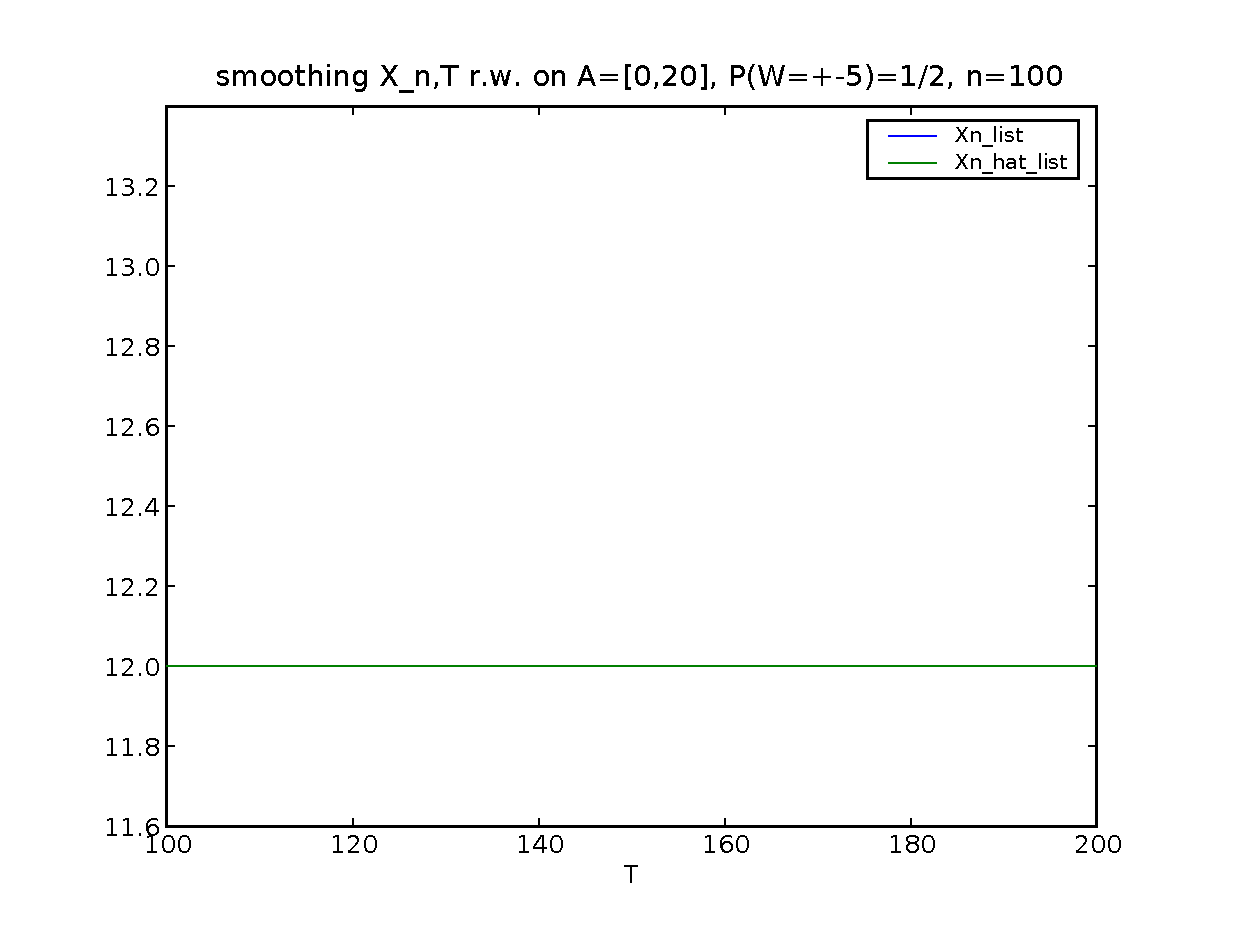
\includegraphics[width=1\textwidth]{hw6_1_a_K_20_L_5_n_100.eps}
\caption{}\label{f1}
\end{figure}

\subsection{No.1 Part b}
Get the prediction estimates of $X_{200}$: $\hat{X_{200,n}}$ for $n=100,...,200$. Plot on the same graph $X_{200}$ and $\hat{X_{200,n}}$. For $L=1$, check Figure~\ref{f2}; for $L=3$, check Figure~\ref{f3}; for $L=5$, check Figure~\ref{f4}; for $L=10$, check Figure~\ref{f5}; for $L=15$, check Figure~\ref{f6}; for $L=18$, check Figure~\ref{f7}; for $L=20$, check Figure~\ref{f8}.

\begin{figure}[p]
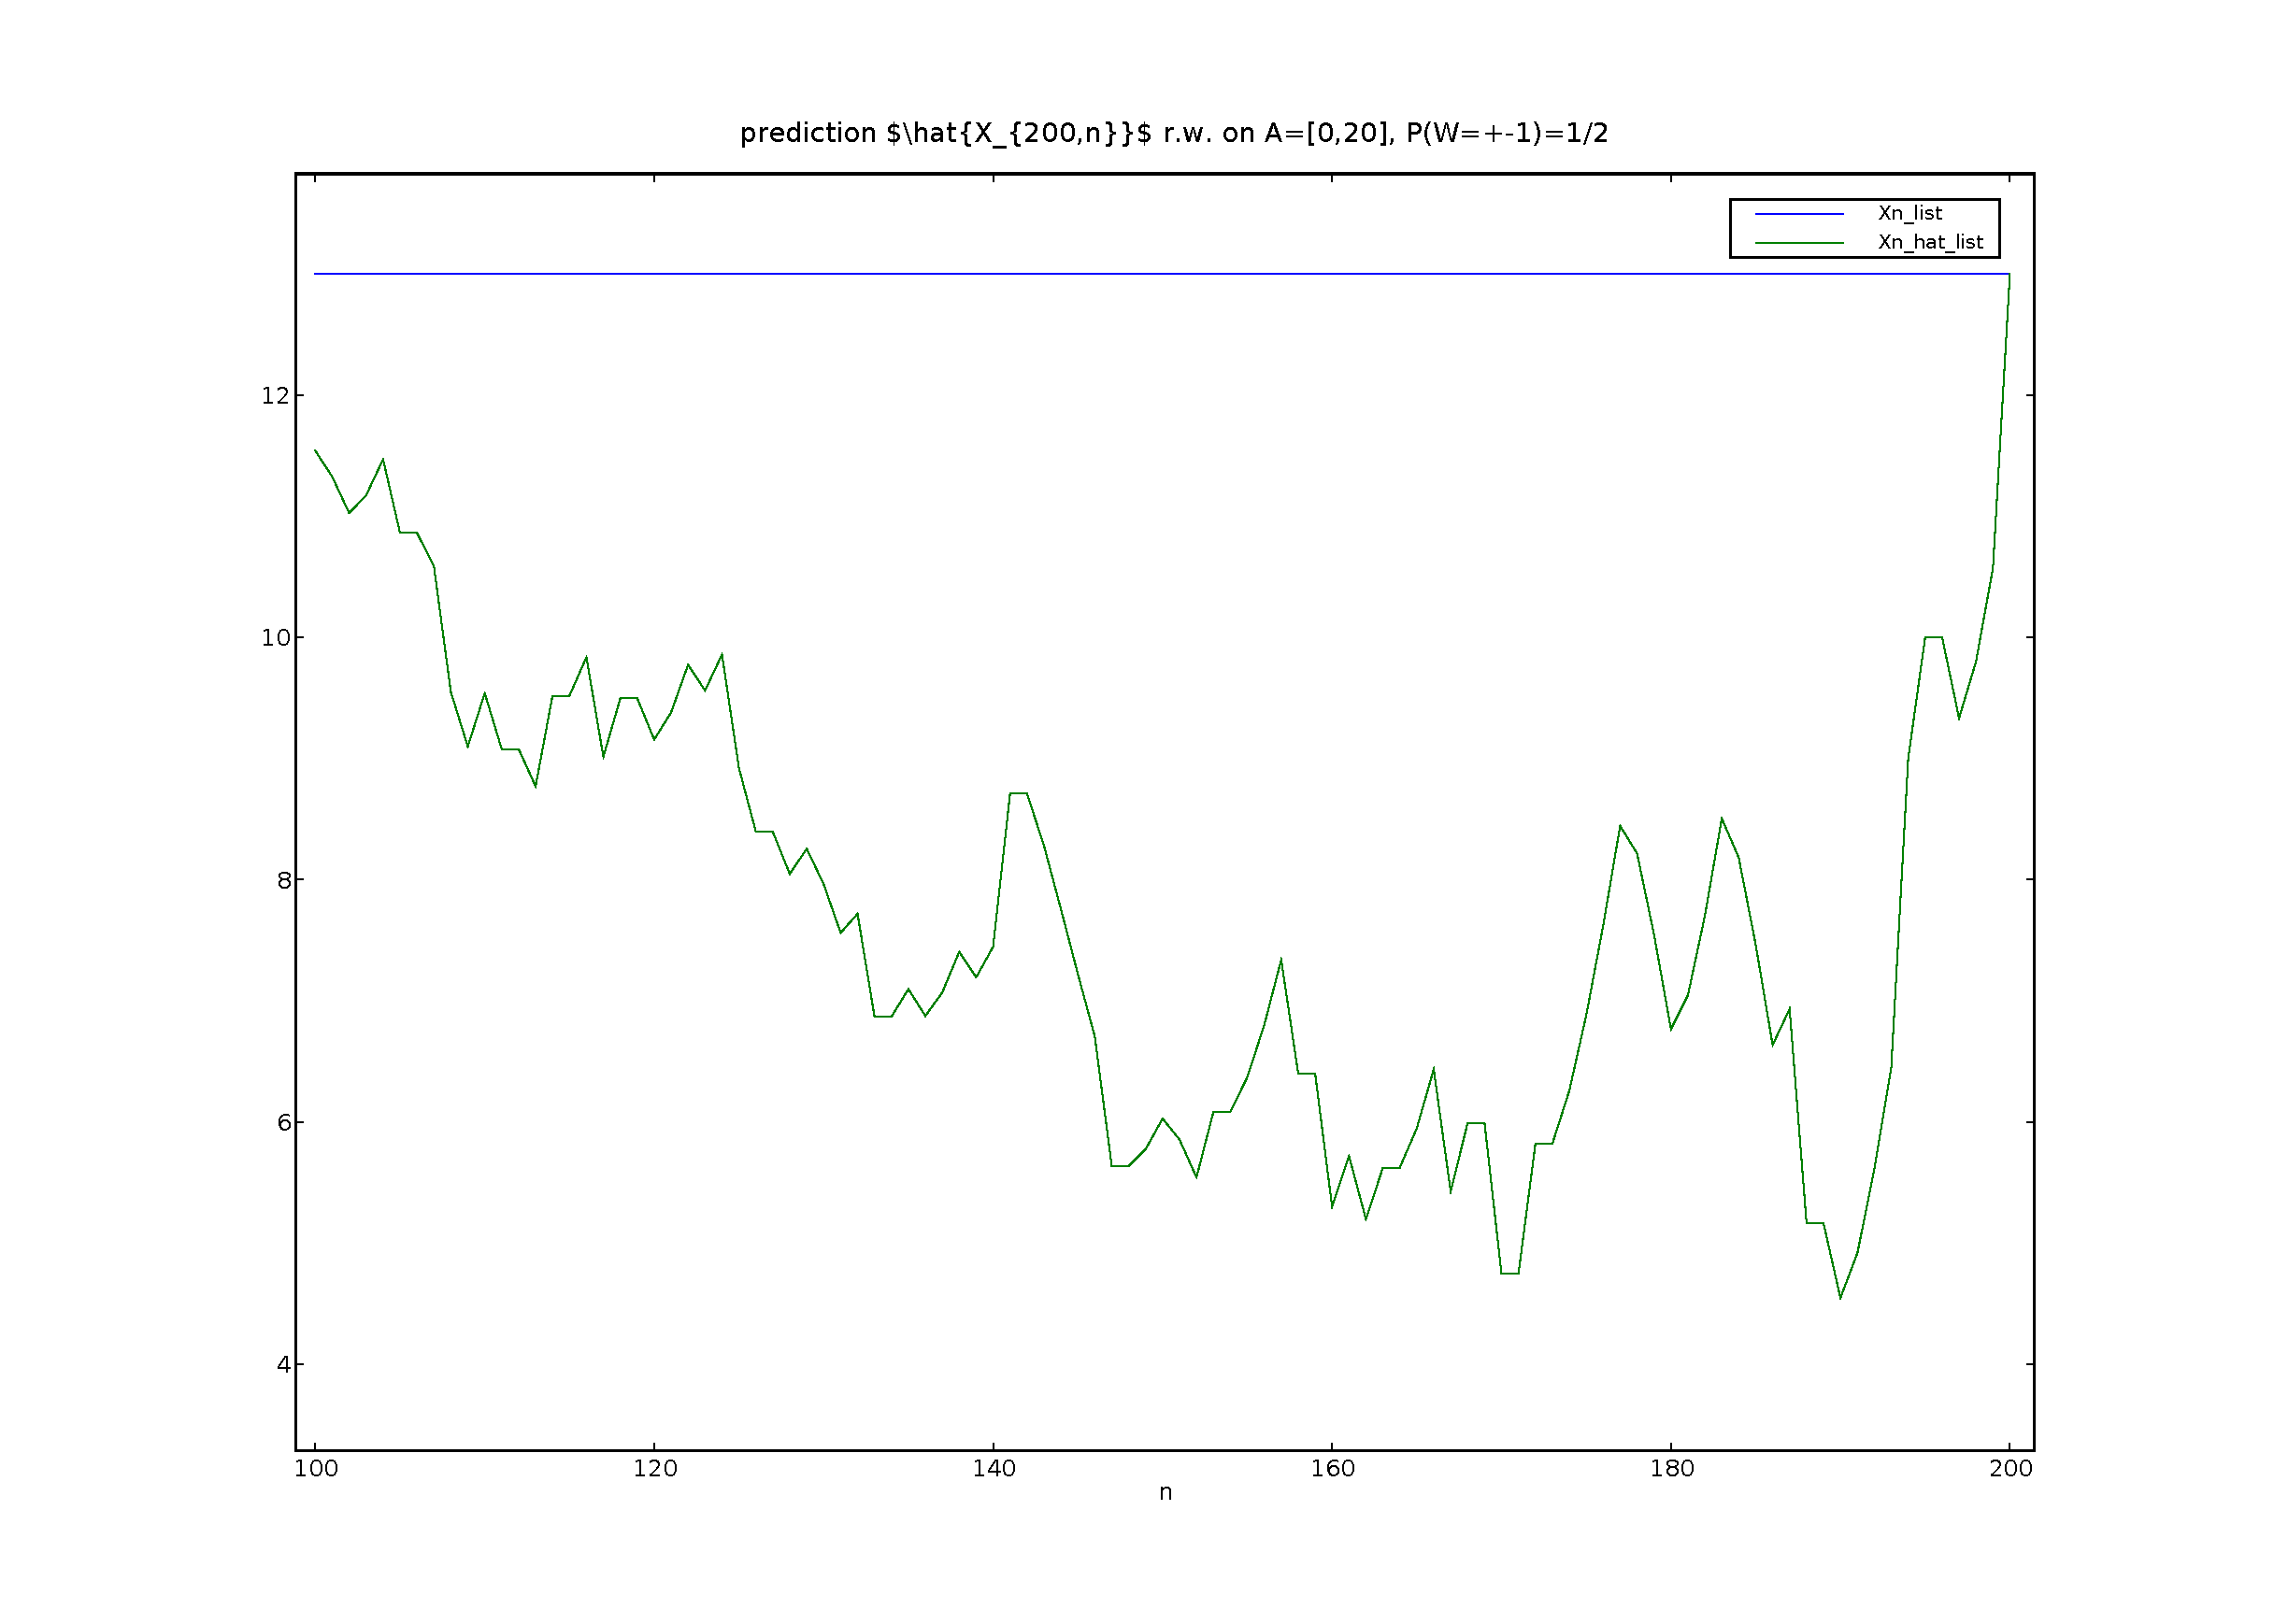
\includegraphics[width=1\textwidth]{hw6_1_b_K_20_L_1_T_200.eps}
\caption{}\label{f2}
\end{figure}

\begin{figure}[p]
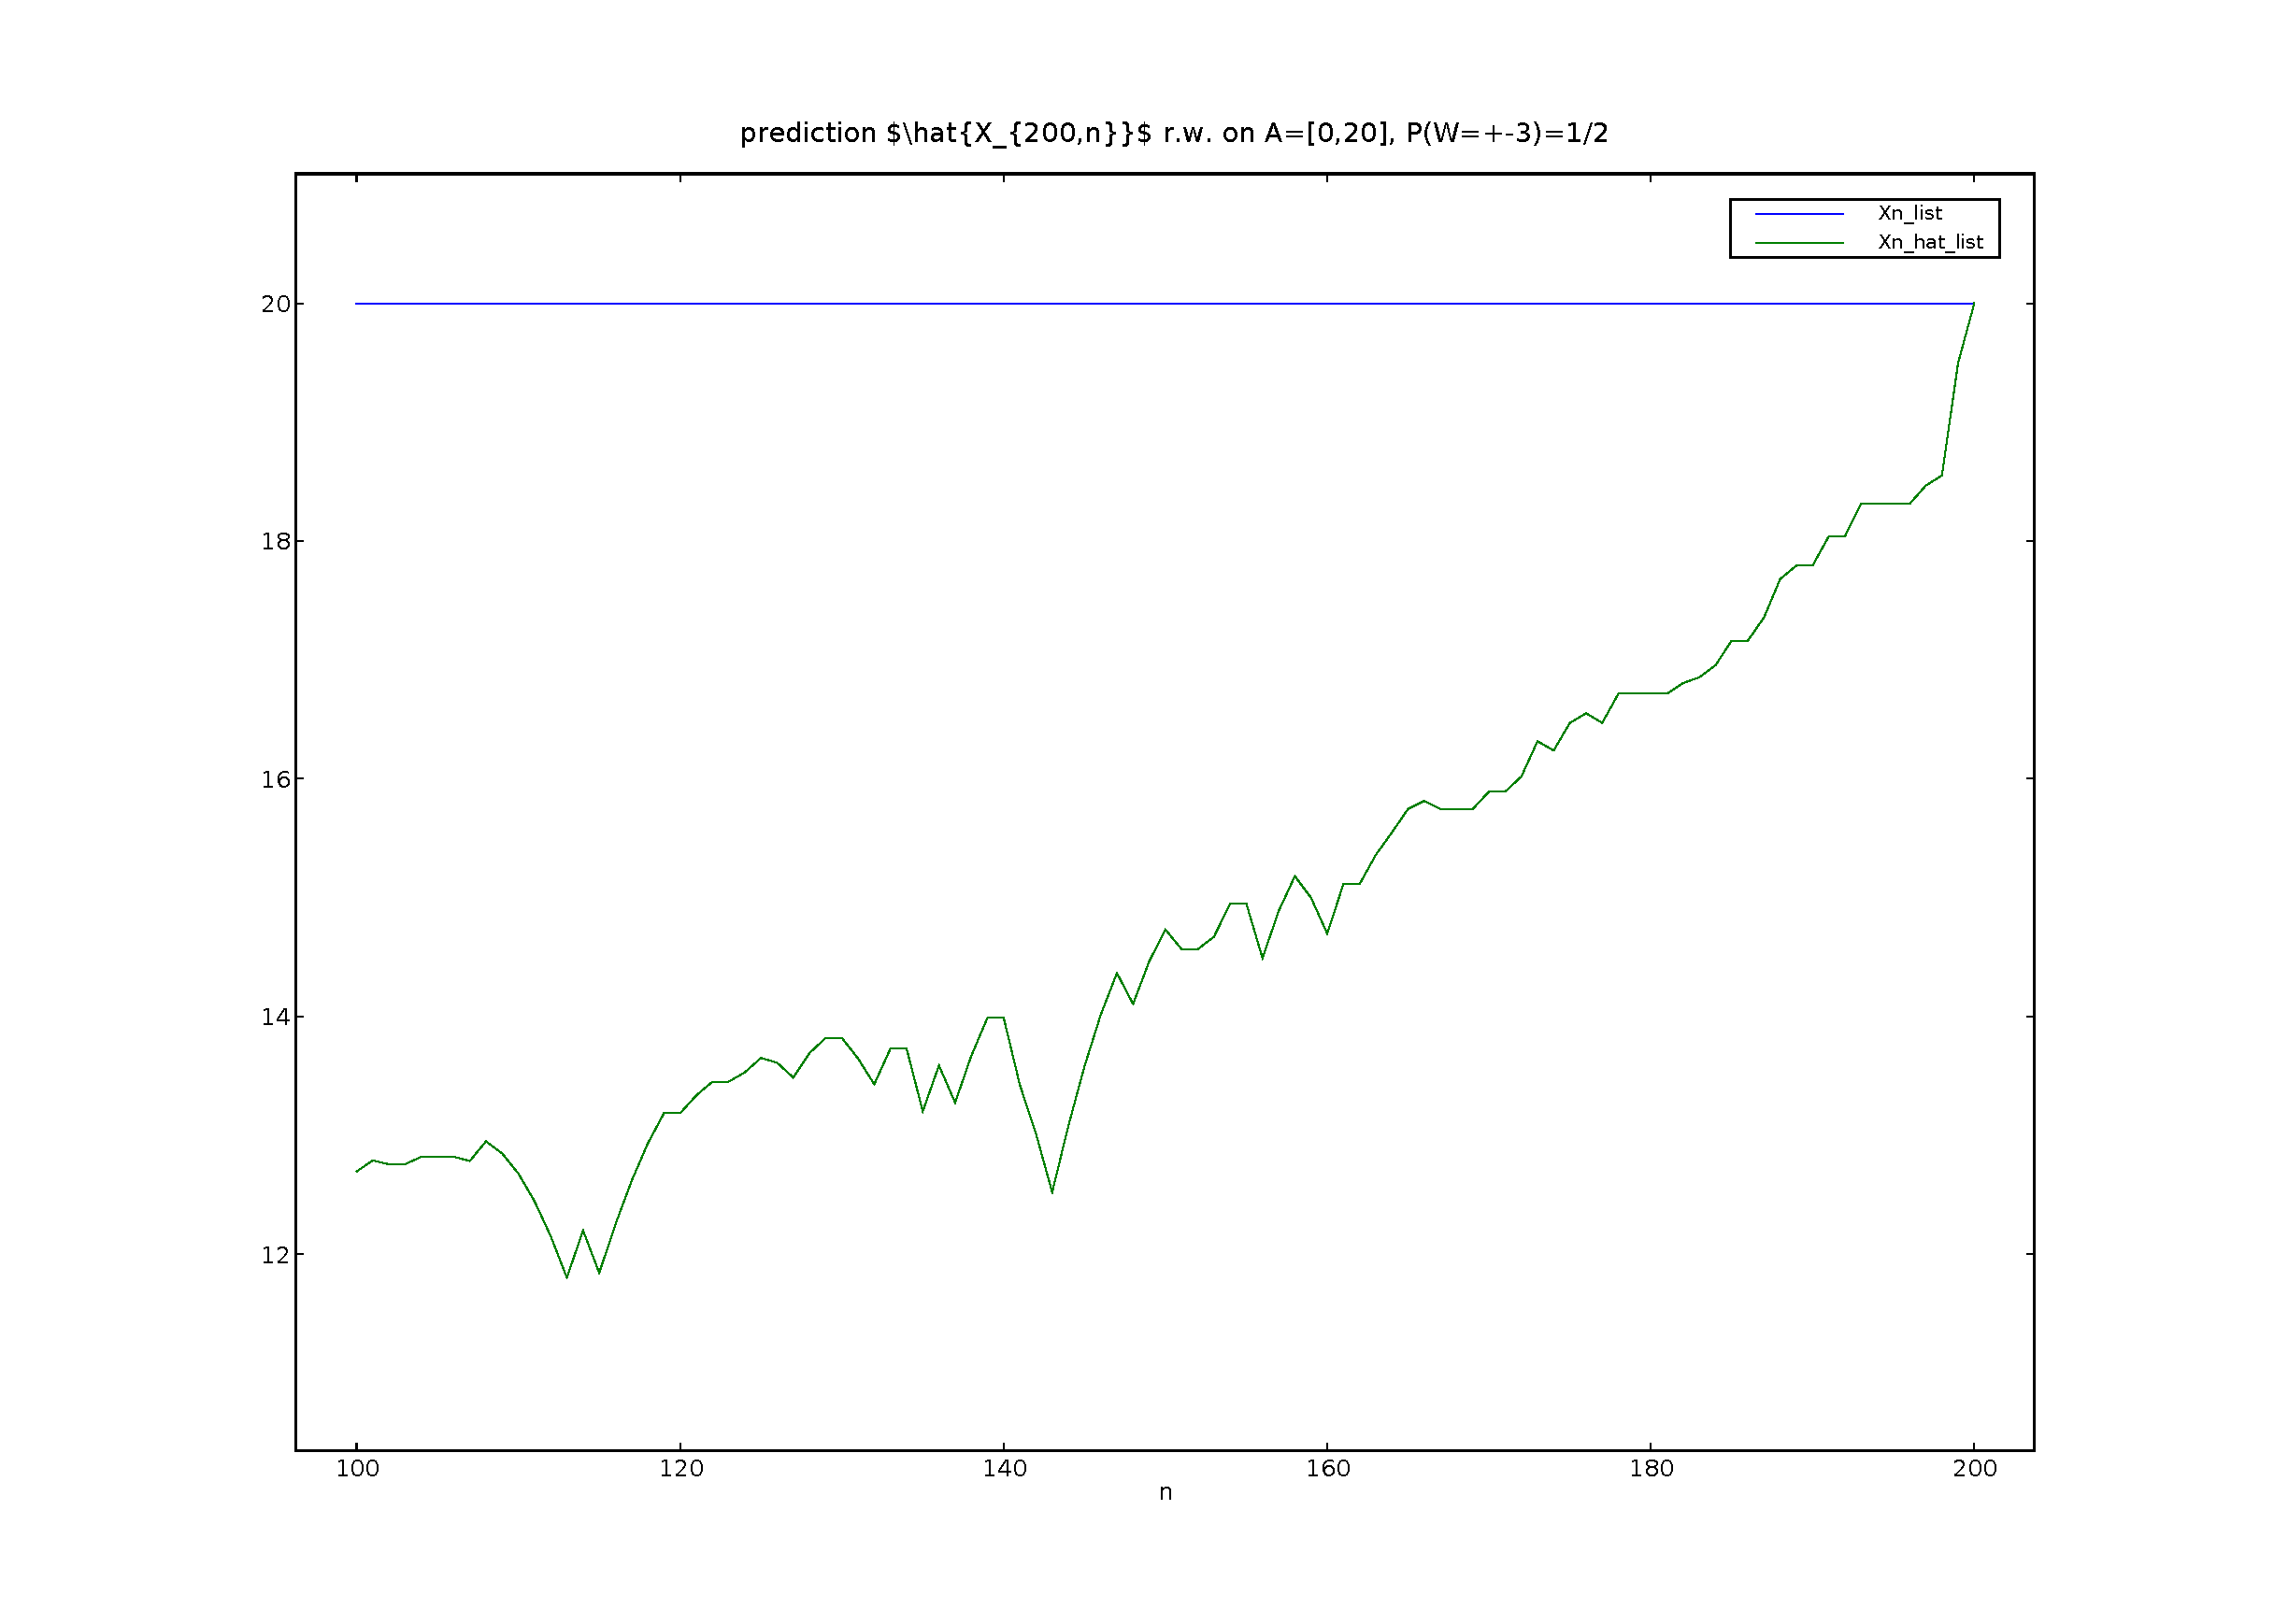
\includegraphics[width=1\textwidth]{hw6_1_b_K_20_L_3_T_200.eps}
\caption{}\label{f3}
\end{figure}

\begin{figure}
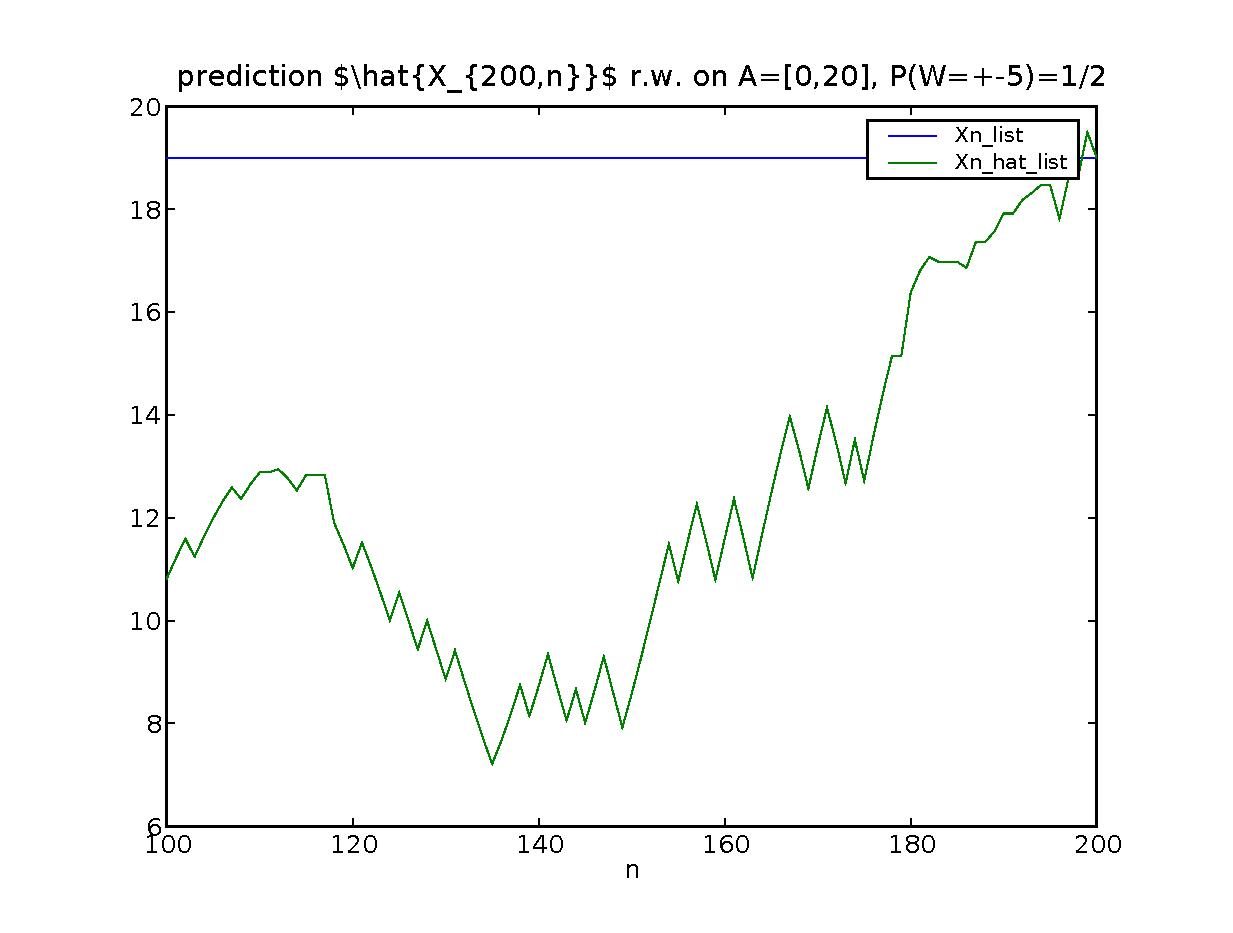
\includegraphics[width=1\textwidth]{hw6_1_b_K_20_L_5_T_200.eps}
\caption{}\label{f4}
\end{figure}

\begin{figure}
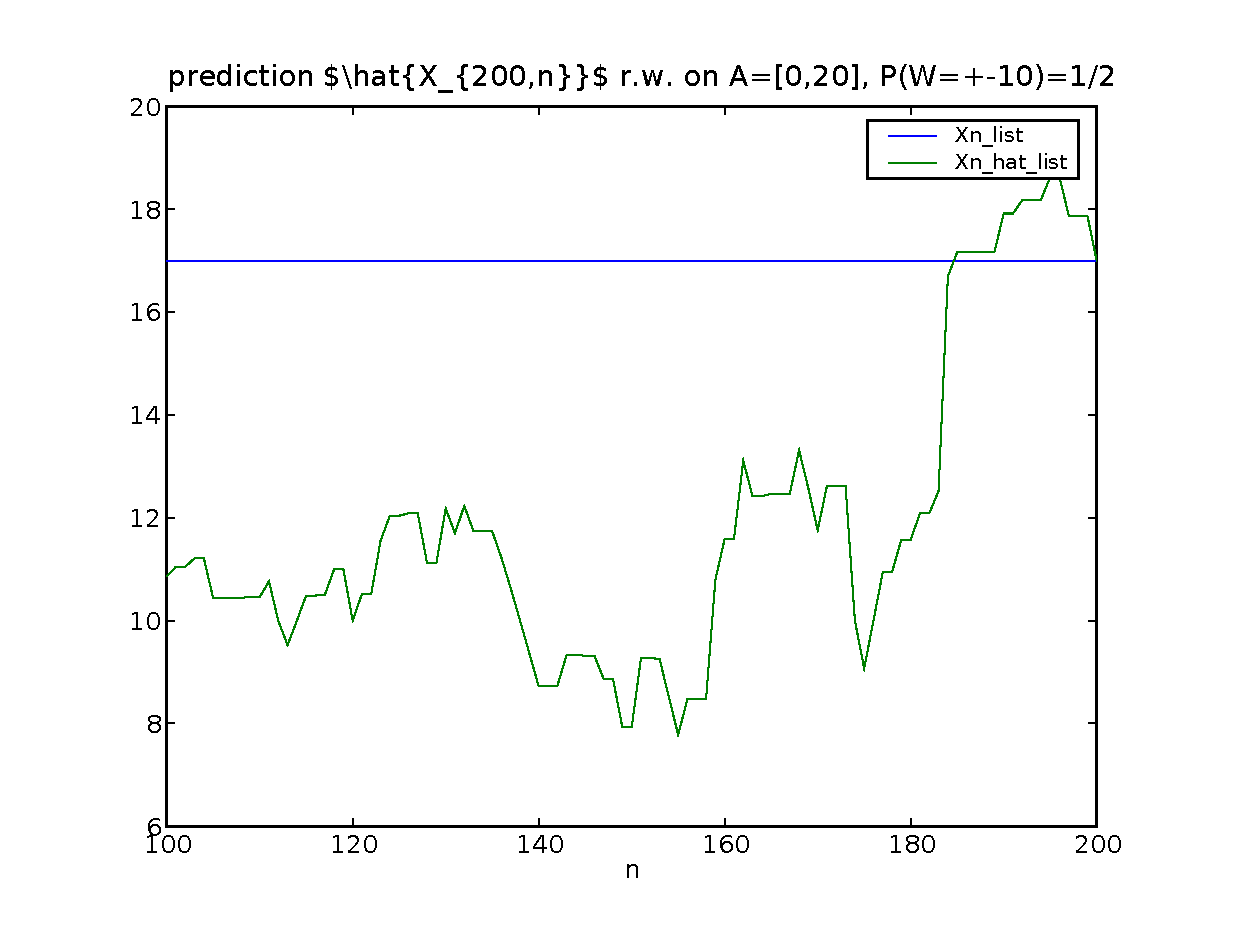
\includegraphics[width=1\textwidth]{hw6_1_b_K_20_L_10_T_200.eps}
\caption{}\label{f5}
\end{figure}

\begin{figure}
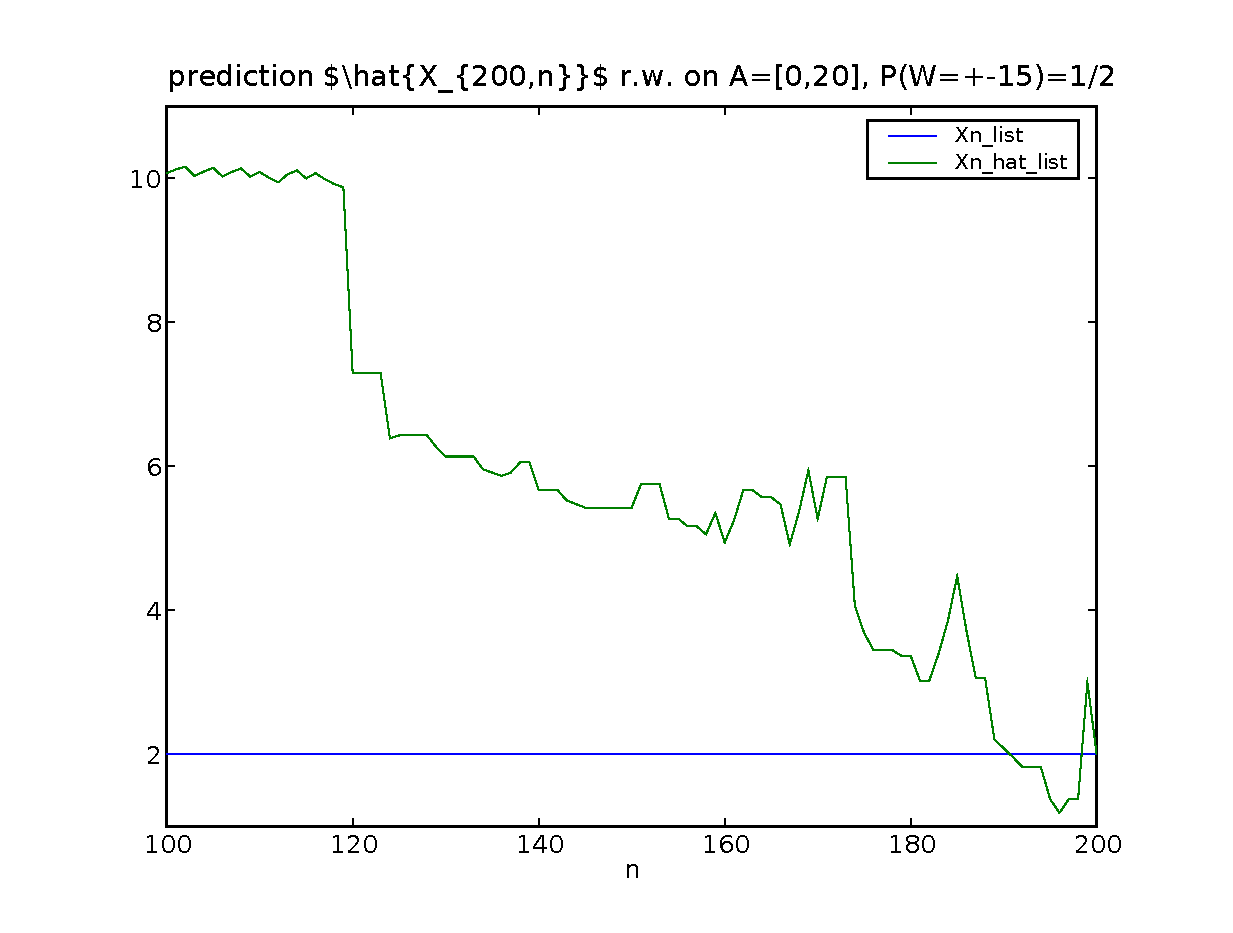
\includegraphics[width=1\textwidth]{hw6_1_b_K_20_L_15_T_200.eps}
\caption{}\label{f6}
\end{figure}

\begin{figure}
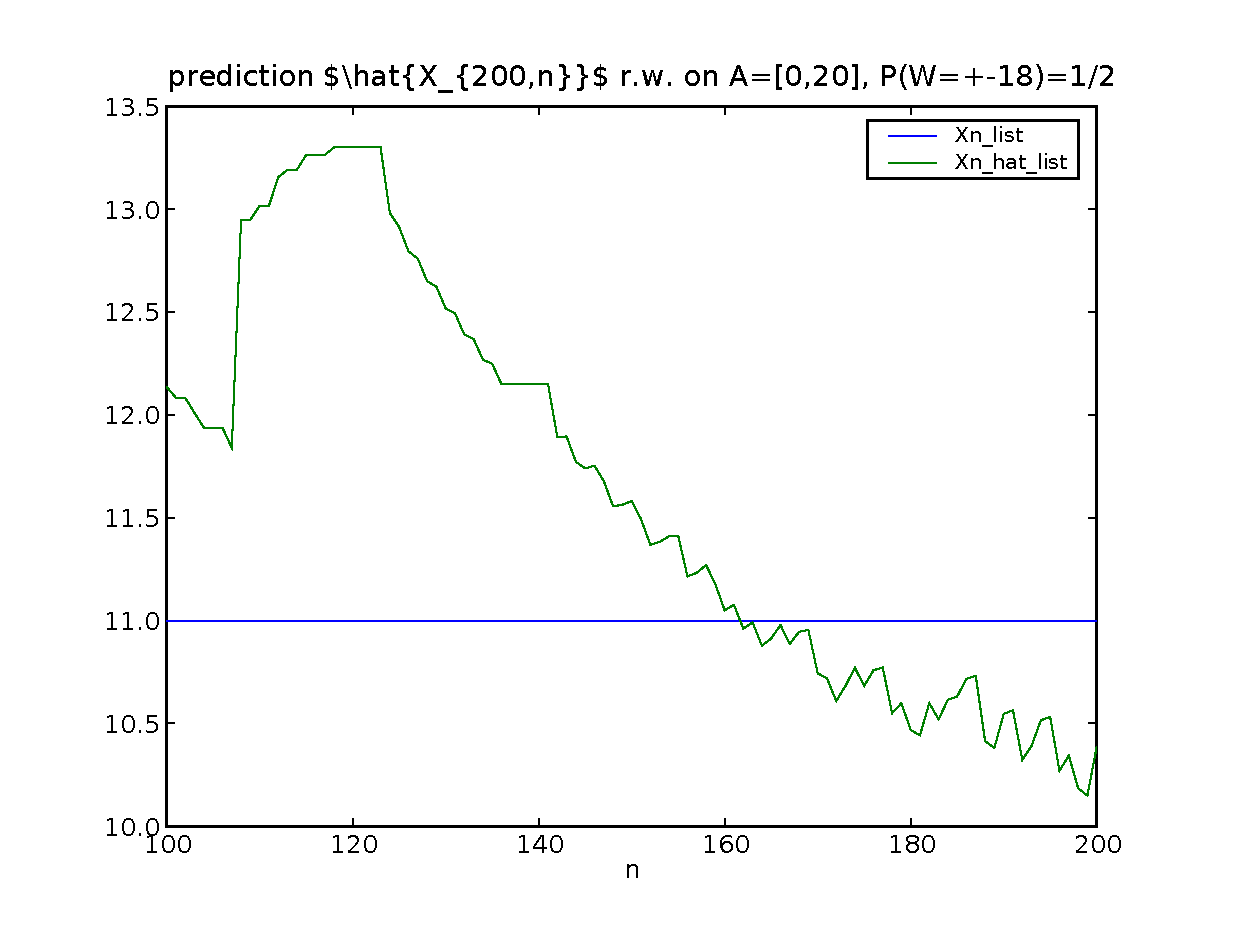
\includegraphics[width=1\textwidth]{hw6_1_b_K_20_L_18_T_200.eps}
\caption{}\label{f7}
\end{figure}

\begin{figure}
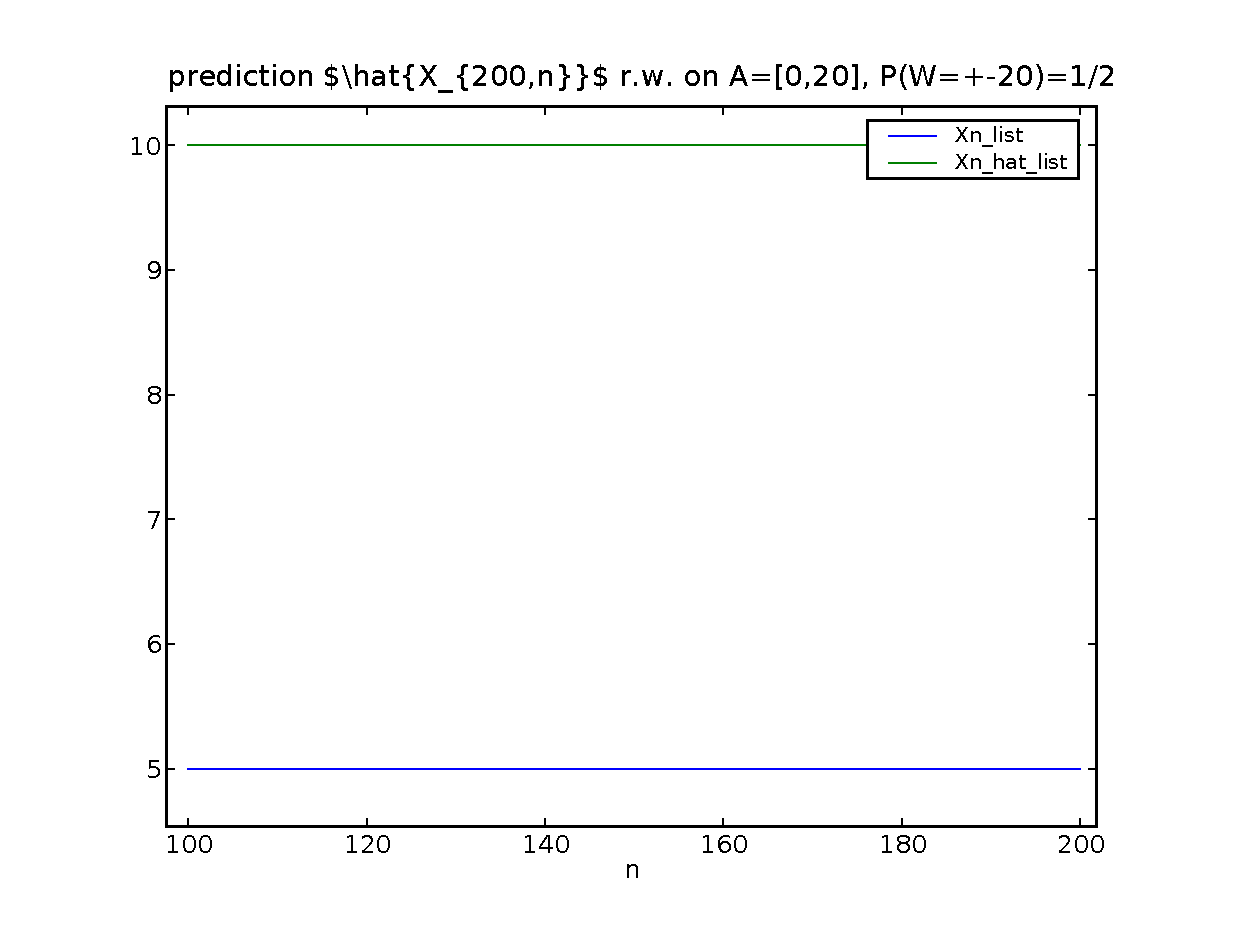
\includegraphics[width=1\textwidth]{hw6_1_b_K_20_L_20_T_200.eps}
\caption{}\label{f8}
\end{figure}

\section{No. 2}
Tossing of coins with initial coin randomly(uniformly) selected. Tossing continues possibly changing the coin with probability $1/3$. Assume we observed $Y_{[0,10]} = HHTHHTHTTTT$.

\subsection{No. 2 Part a, Smoothing}
Find $P(X_5 = i | Y_{[0,8]})$ and $P(X_5 = i | Y_{[0,10]})$, $i=1,2,3$. Here is the answer. The 1st row is $Y_{[0,8]}$ and 2nd row is $Y_{[0,10]}$. The columns correspond to $i=1,2,3$. It looks like future information doesn't help in the smoothing. The reason is that the backward equation $\mu^i_n(b_{[n+1,T]})$ has same value for different $i$ regardless of $n$.

\begin{verbatim}
[[ 0.46666667  0.33333333  0.2       ]
 [ 0.46666667  0.33333333  0.2       ]]
\end{verbatim}


\subsection{No. 2 Part b, Prediction}
Find $P(X_{10} = i | Y_{[0,5]})$ and $P(X_{10} = i | Y_{[0,6]})$, $i=1,2,3$. Here is the answer. The 1st row is $P(X_{10} = i | Y_{[0,5]})$ and 2nd row is $P(X_{10} = i | Y_{[0,6]})$. The columns correspond to $i=1,2,3$. It seems the observation has no power in terms of prediction. The reason is that the transition matrix of X, $P^n(X_i,X_j)$ doesn't change with $n$.

\begin{verbatim}
[[ 0.33333333  0.33333333  0.33333333]
 [ 0.33333333  0.33333333  0.33333333]]
\end{verbatim}


\end{document}
